\documentclass[ignorenonframetext,hyperref={pdftex,unicode}]{beamer}
%\documentclass[aspectratio=169,ignorenonframetext,hyperref={pdftex,unicode}]{beamer}  %соотношение 16:9

\usepackage{amssymb,amsmath,mathtext} %поддержка формул и русского текста в них
\usepackage{indentfirst,amsfonts} %поддержка русского стиля оформления текста и формул
%\usepackage{makecell,multirow,longtable} %поддержка таблиц занимающих несколько страниц

\usepackage[english,russian]{babel}
\usepackage[T2A]{fontenc}
\usepackage[utf8]{inputenc} %кодировка исходника

% for hyperlinks
\usepackage{hyperref}
% for strike-out text
\usepackage[normalem]{ulem}

\ifpdf
        \usepackage{cmap} % чтобы работал поиск по PDF
        %\usepackage[pdftex]{graphicx}
        \pdfcompresslevel=9 % сжимать PDF
\else
        \usepackage{graphicx}
\fi

\usetheme{Samsolutions} %корпоративная тема

%\setbeamercovered{transparent} %полупрозрачные скрытые элементы

\title{Як мы ставілі KDE пад FreeBSD} %название презентации
%\subtitle{SUBTITLE} %подназвание
\author["Андрэй Захарэвіч"]{Андрэй Захарэвіч\\ andrej@zahar.ws} %автор


\begin{document} %начало документа

\frame{\titlepage} % Создание заглавной страницы


\section{Мэты і пачатковы статус} %названия секций для оглавления

\begin{frame}{Што мы хацелі атрымаць} %новый слайд и его название
	Стала цікава атрымаць нешта кшталту дэсктопа на FreeBSD. Паколькі мы выкарыстоўвалі XFCE+i3 і Gnome3+Unity, хацелася б:
	\begin{itemize}
		\item Загрузка ў графічнае асяроддзе пры старце сістэмы (з лагінам, але без дадатковых кансольных дзеянняў)
		\item Нейкі працоўны стол з якім мы не працуем пастаянна
	\end{itemize}
	\begin{center}
 		
\includegraphics[height=0.5\textheight,keepaspectratio]{freebsd_badge} %так вставляется картинка
	\end{center}
\end{frame} %конец слайда

\begin{frame}{Што мы мелі} 
	Апроч жадання эксперыментаваць:
	\begin{itemize}
		\item Загрузачны DVD з інсталяком апошняй (10.1) версіі FreeBSD
		\item Некаторы досвед Linux на дзве персоны
		\item Крыху энтузіазма
		\item Доступ у інтэрнэт праз знакамітую проксі { }
\includegraphics[height=2em,keepaspectratio]{SaMLogo}
	\end{itemize}
\end{frame} %конец слайда

\section{Працэс інсталяцыі і настройкі}
\begin{frame}{Інсталяцыя FreeBSD} %новый слайд и его название
	Нічога складанага ці немагчымага. Базавую сістэму з ZFS можна лёгка і хутка паставіць нават не чытаючы афіцыйнае кіраўніцтва.
	\begin{center}
 		
\includegraphics[height=0.5\textheight,keepaspectratio]{338391435_f1e7094228_z} %так вставляется картинка
	\end{center}
\end{frame} %конец слайда

\begin{frame}{Інсталяцыя KDE: першая спроба} %новый слайд и его название
	Паколькі дакументацыя FreeBSD настойліва раіць выкарыстоўваць \texttt{pkg} для інсталяцыі, пачнем:

	\texttt{\# pkg install kde}
	\begin{center}
 		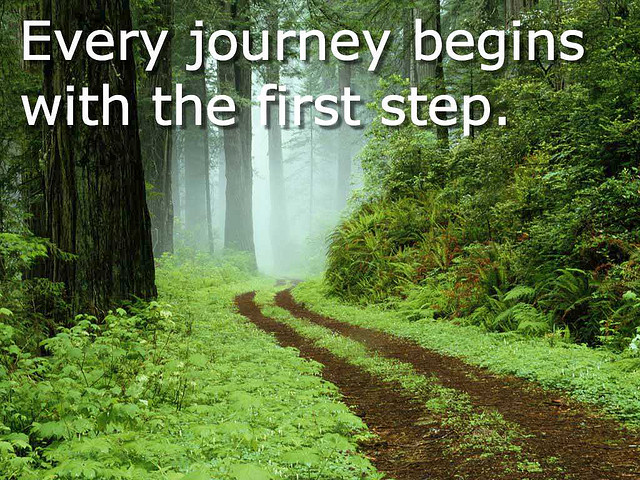
\includegraphics[height=0.7\textheight,keepaspectratio]{2656648042_0ced853512_z} %так вставляется картинка
	\end{center}
\end{frame} %конец слайда

\begin{frame}{Інсталяцыя KDE: першая праблема} %новый слайд и его название
	І нічога не адбываецца. Наогул. Праз пяць хвілін чакання да нас пачынае даходзіць, што нешта не тое.
	\begin{center}
 		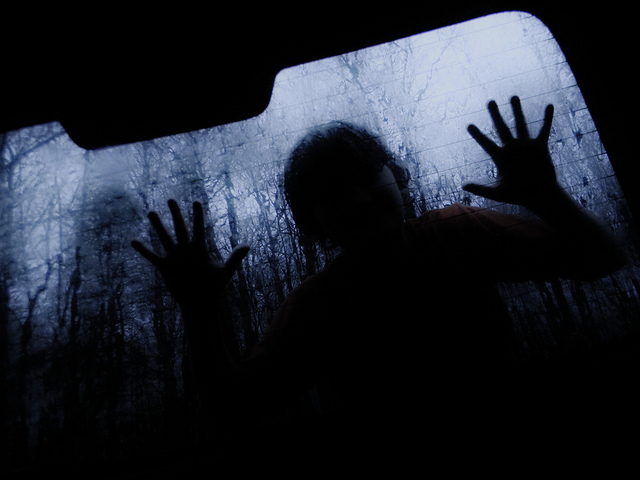
\includegraphics[height=0.7\textheight,keepaspectratio]{6428406857_0f97c985fd_z} %так вставляется картинка
	\end{center}
\end{frame} %конец слайда

\begin{frame}{Інсталяцыя KDE: пайшла вада ў хату} %новый слайд и его название
	Мы забыліся прапісаць знакамітую проксі { }
\includegraphics[height=2em,keepaspectratio]{SaMLogo}.

	Выпраўляем памылку:

	\texttt{\# setenv http\_proxy <адрас:порт>}

	\texttt{\# pkg install kde}

	\begin{center}
 		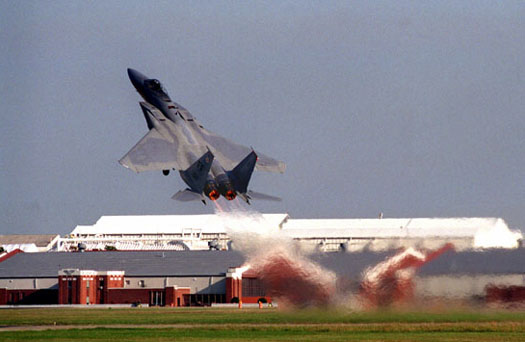
\includegraphics[height=0.6\textheight,keepaspectratio]{F-15_takeoff} %так вставляется картинка
	\end{center}
\end{frame} %конец слайда

\begin{frame}{Інсталяцыя KDE: безсэнсоўны поспех} %новый слайд и его название
	І вось тут KDE і паставіцца. Прычым, заўважце, у адрозненне ад Debian, тут пакетны манэджэр сам, без нагадвання, абновіць сваю базу дадзеных. Безумоўна, падцягне і залежнасці, сярод якіх:
	\begin{itemize}
		\item subversion;
		\item mysql-client;
		\item mysql-server;
		\item gtk2;
		\item ImageMagick.
	\end{itemize}
Але ніякіх X, Wayland ці іншых адпаведных сістэм. 
	\begin{center}
 		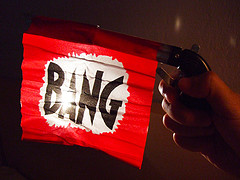
\includegraphics[height=0.3\textheight,keepaspectratio]{914441359_f509440169_m} %так вставляется картинка
	\end{center}
\end{frame} %конец слайда

\begin{frame}{Інсталяцыя X} %новый слайд и его название
	Што мы можам зрабіць, апроч як:

	\texttt{\# pkg install xorg}
	
	І пасля інсталяцыі мы ўжо нават можам запусціць іксы. Але там пакуль проста голы стол і некалькі тэрміналаў.
	\begin{center}
 		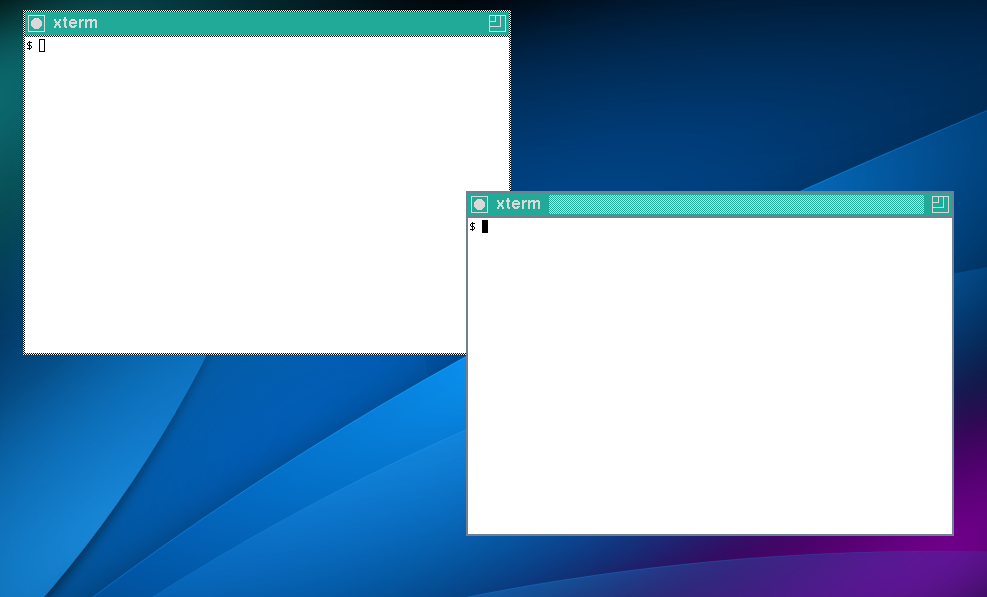
\includegraphics[height=0.6\textheight,keepaspectratio]{TWM} %так вставляется картинка
	\end{center}
\end{frame} %конец слайда

\begin{frame}{Настройка загрузкі KDM} %новый слайд и его название
	Я б прапанаваў паставіць які больш мацёры рэдактар, чым чысты vi, але гэта, безумоўна, неабавязкова

	\texttt{\# pkg install nano vim}
	\\~\\	
	І пасля інсталяцыі (ці замест яе) дадаем у скрыпт \texttt{/etc/rc.conf} наступныя радкі:

	\texttt{dbus\_enable="YES"}
	
	\texttt{kdm4\_enable="YES"}
\end{frame} %конец слайда

\begin{frame}
	Пасля чаго будзе дастаткова адной перазагрузкі.
	\begin{center}
 		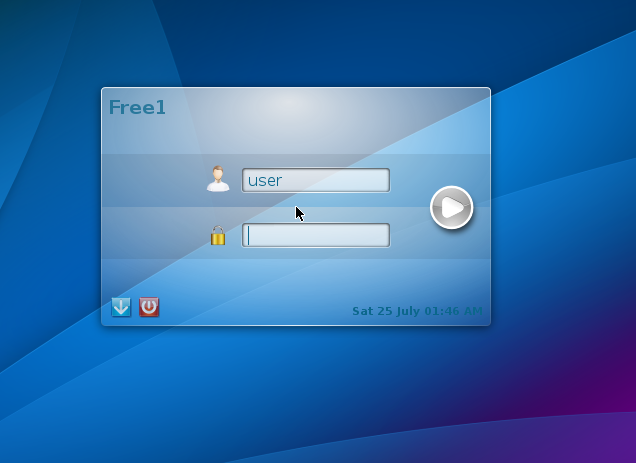
\includegraphics[height=0.8\textheight,keepaspectratio]{KDM} %так вставляется картинка
	\end{center}
\end{frame}

\frame{\finalslide{Пытанні?}} %слайд вопросы?

\begin{frame}{Ужытыя малюнкі}
	\begin{thebibliography}{10}
	\beamertemplatetextbibitems
	\bibitem{}
		{\sc \href{http://amai-biscuit.deviantart.com/art/FreeBSD-Badge-345132138}{FreeBSD Badge}} by {\sc \href{http://amai-biscuit.deviantart.com/}{amai-biscuit}};
	\bibitem{}
		{\sc \href{https://www.flickr.com/photos/nmcmanus/338391435}{Easy Button}} by {\sc \href{https://www.flickr.com/photos/nmcmanus/}{Civilian Scrabble}};
	\bibitem{}
		{\sc \href{https://www.flickr.com/photos/martinaphotography/6428406857}{66/365 Another Creepy One}} by {\sc \href{https://www.flickr.com/photos/martinaphotography/}{martinak15}};
	\bibitem{F-16}
		{\sc \href{https://commons.wikimedia.org/wiki/File:F-15\_takeoff.jpg}{F-15\_takeoff}} by {\sc USAF};
	\bibitem{}
		{\sc \href{https://www.flickr.com/photos/toasty/914441359}{Bang!}} by {\sc \href{https://www.flickr.com/photos/toasty/}{Kenneth Lu}}.
	\end{thebibliography}
\end{frame}

\end{document}
